\documentclass[12pt, a4paper, oneside]{book}


\usepackage[italian]{babel}
\usepackage[T1]{fontenc}
\usepackage{amsthm}
\usepackage{amsmath}%
\usepackage{amsfonts}%
\usepackage{amssymb}%
\usepackage{graphicx}
\usepackage[utf8]{inputenc}
\usepackage{float}
\usepackage{url}
\usepackage{cite}


\usepackage{algorithm}
\usepackage{algpseudocode}

\usepackage{tkz-graph}  
\usepackage{tikz}
\usetikzlibrary{shapes.geometric, arrows}
\usetikzlibrary{arrows.meta}
\usetikzlibrary{decorations.pathreplacing}
\linespread{1.3}

\newtheorem{mydef}{Definition}
\newtheorem{theorem}{Theorem}
\newtheorem{observation}{Observation}
\newtheorem{corollary}{Corollary}
\newtheorem{proposition}{Preposition}
\newtheorem{lemma}{Lemma}
\newtheorem{example}{Example}


\usepackage[top=3.5cm, bottom=3.5cm, left=4cm, right=3.5cm]{geometry}


\renewcommand{\vec}{\bm}
\begin{document}

\tableofcontents
\pagenumbering{arabic}

\newpage
\thispagestyle{empty}
\listoffigures

\newpage
\thispagestyle{empty}
\section*{abstract}
Questa tesi si occupa di presentare le metodologie e strumenti applicati nella realizzazione di una etichettatrice di flaconi ad alta velocità progettata e sviluppata per l'area farmaceutica.
Verranno spiegati i processi necessari allo sviluppo software sia per quanto riguarda la parte PLC che la parte SCADA/HMI nonche quella relativa allo sviluppo del sistema di Visione e controllo.
Si analizzeranno i vari dispositivi che compongono il macchinario, il loro funzionamento ed in particolar modo i protocolli di comunicazione che ci permettono di dialogare con essi. 
Verrà affrontata inoltre la tematica dell'Industria 4.0 spiegando come poter sviluppare un sistema software che rispetti i criteri del nuovo standard nell'automazione Industriale.
 

\newpage
\thispagestyle{empty}
\section*{Introduzione al progetto}
Spiegare la necessita di costruzione di una macchina dalle dimensioni ridotte veloce e affidabile. 

\chapter{Etichettatrice RMC17002}
In questo capitolo spiegheremo il funzionamento dell'Etichettatrice ma è necessario partire prima da una breve descrizione sulla struttura meccanica per poi passare ad una dettagliata analisi dei dispositivi Elettrici ed Elettronici che la compongono.
\section{Struttura Meccanica}
Dettagli meccanici - Dimensione -Elementi(Natsro in e out) - stella ingresso,centrale,scarto - raccoglitore Scarto - guide regolabili per dispositivi - struttura di acciaio con porte di plexiglass
\section{Dispositivi Elettrici ed Elettronici}
Dispositivi Elettrici ed elettronici
\section{Funzionamento del Macchinario}
Prima di spiegare il funzionamento dettagliato del macchinario, conviene introdurre brevemente il suo funzionamento base. Per semplificare il tutto dividerò a fasi il processo di etichettaggio.

Il funzionamento base del macchinario è abbastanza semplice. 
\begin{itemize}
	\item \textit{Ingresso Flaconi} All ingresso alla nostra etichettatrice abbiamo un nastro trasportatore che arriva dalla macchina precedente che nel caso di questa linea è una macchina riempitrice.
	\item \textit{Controllo Presenza}  I flaconi uscenti dalla riempitrice scorrono sul nastro fino al raggiungimento della prima stella. Durante il trasporto nella prima stella, ogni flacone viene rilevato dal sensore di presenza prodotto.
	\item \textit{Etichettatura} Successivamente il flacone viene agganciato dalla seconda stella che lo trasporta sull'unità di etichettaggio. Quando il flacone si trova in prossimità della "pinna", viene attivata la testa di etichettatura che effettuerà l'applicazione.
	\item \textit{Massaggio} Quasi istantaneamente all'applicazione, il flacone rotola su un nastro detto massaggiatore che assicura una corretta attaccatura dell'etichetta.
	\item \textit{Uscita Flacone} A questo punto il flacone viene agganciato dalla terza ed ultima stella che lo trasporta sul nastro di uscita verso la macchina a valle. 
\end{itemize}

Avendo sommariamente illustrato il funzionamento base della nostra etichettatrice tralasciando controlli, sistemi di visione, meccanismi di scarto ed altro, andiamo ora a spiegare un po più nel dettaglio cosa avviene realmente in ogni fase.

\subsection{Ingresso Flaconi}
Nella fase di ingresso flaconi, come si può ben immaginare non vi è solo un semplice nastro che trasporta i flaconi da un punto ad un altro bensì vi sono alcuni controlli necessari per un corretto funzionamento del macchinario nonchè di protezione del sistema stesso. Prima di tutto il nastro in ingresso è regolabile in velocità mediante un inverter per assicurare che i flaconi arrivino con una giusta frequenza. \textcolor{red}{FIGURA} Non manca sul nastro in ingresso il sensore di minimo carico che segnala il plc qualora non ci sia prodotto. Alla ricezione di tale segnale il plc provvederà a fermare la macchina che altrimenti girerebbe inutilmente (vi sono inoltre anche segnali di abilitazione che arrivano dalla macchina a monte necessari a segnalare un interruzione della linea).
Un problema non da sottovalutare nella nostra applicazione è la possibilità che un flacone si rovesci su nastro o arrivi già rovesciato dalla macchina a monte (mai fidarsi di chi si ha prima). Un flacone rovesciato potrebbe essere estremamente pericoloso, se la stella alla fine del nastro dovesse mai agganciare un flacone di vetro mal posizionato lo farebbe in mille pezzi e richierebbe di danneggiare la macchina. Per evitare ciò, abbiamo munito il minimo carico di doppio sensore (uno alto ed uno basso). \textcolor{red}{FIGURA} Questi due sensori lavorano in contemporanea uno sopra l'altro in modo tale che se un flacone dovesse passare rovesciato, solo il sensore basso ne rileverebbe la presenza. Questa situazione manda un allarme che blocca immediatamente la macchina avvisando l'operatore mediante HMI.  
   
\subsection{Controllo Presenza}
In questa fase che sembra la più banale inizia il vero fulcro del controllo che si porterà avanti per tutto il processo. Il flacone viene agganciato dalla prima stella e durante il trasporto il sensore di presenza ne verifica la presenza. 
Questo momento è cruciale perchè è quì che si attiva lo "Shift Register" del controllo che vedremo in dettaglio nei capitoli successivi. Per ora anticipiamo lo "Shift Register" come l'elemento che ci permette di determinare la posizione e lo stato di ogni flacone all'interno della macchina.
\subsection{Etichettatura}
Sicuramente la Fase più importante di tutto il processo, l'etichettatura è anche la più complessa a livello di controlli e settaggio. Il flacone una volta rilevato dal sensore di presenza, viene agganciato dalla seconda stella che lo trasporta sulla pinna di etichettatura. Una volta che il flacone si trova in prossimità della pinna (Camme programmate su giri macchina \textcolor{red}{riferimento capitolo}) viene inviato un comando di trigger digitale alla testa di etichettatura che applicherà l'etichetta. 


 
Racconto dettaglato del processo dall'ingresso dei flaconi all'uscita passando tra i vari controlli.
\chapter{Processo di Sviluppo software PLC}
Un \textit{PLC} è, in pratica, un controllore programmabile, dotato di ingressi e uscite analogiche e digitali, con una o più connessioni di reti e specializzato nella gestione dei processi industriali. Il PLC esegue un programma ed elabora i segnali digitali ed analogici provenienti dai sensori ricevuti attraverso gli ingressi, generando sulle proprie uscite i corrispondenti comandi per gli attuatori presenti in un impianto industriale, i quali riescono a gestire una moltitudine di funzioni dalla più elementare (rilevare la temperatura, accendere una lampadina, etc) alle più sofisticate e complesse (muovere un braccio meccanico, programmare l’accensione/avviamento di macchine, automi, ecc). 
I PLC sono di solito istallati in armadi nelle vicinanze dell'impianto o direttamente a bordo della macchina. Gli I/O possono essere remoti: in questo caso sono collegati a morsettiere che vengono messe in comunicazione con il PLC mediante "bus di campo" o anche direttamente su Ethernet. Sono necessarie postazioni utilizzate dagli operatori per "vedere" e capire cosa succede negli impianti, dato che i PLC sono dei dispositivi "ciechi" non dotati di interfaccia di visualizzazione.
\\La prima azione che il PLC compie è la lettura degli ingressi del portale e si intende tutti gli ingressi sia digitali sia analogici, on board o su bus di campo (schede remote collegate al PLC o con una rete di comunicazione). Dopo aver letto tutti gli ingressi, il loro stato viene memorizzato in una memoria che è definita "\textit{Registro immagine degli ingressi}". A questo punto le istruzioni di comando vengono elaborate in sequenza dalla CPU e il risultato viene memorizzato nel "\textit{Registro immagine delle uscite}". Infine, il contenuto dell'immagine delle uscite viene scritto sulle uscite fisiche, ovvero le uscite vengono attivate. Poiché l'elaborazione delle istruzioni si ripete continuamente, si parla di elaborazione ciclica; il tempo che il controllore impiega per una singola elaborazione viene detto tempo di ciclo (solitamente da 10 a 100 millisecondi).
\section{Fase Iniziale }
Si parte dalla attenta analisi degli schemi elettrici della macchina (FOTO SCHEMA ELETTRICO)
Scelta tool e TIA PORTAL

\section{Best Practices}
spiegazione delle best practice sul come strutturare un software PLC REMAPPING I/O, utilizzo di FB per dispositivi esterni (MOTORI MITSUBISHI - TELECAMERE DATALOGIC - ENCODER MACCHINA - STAMPANTE - NORMALIZZAZIONI) GSD
\section{Comunicazione Con Dispositivi Macchina}

\section{Camme Digitali e Sistemi di Controllo}
Per spiegare cosè una Camma digitale conviene descrivere prima la classica camma meccanica. Sebbene le due hanno utilizzi diversi, alcuni principi rimangono gli stessi.

La camma meccanica è un elemento di forma eccentrica calettato su un asse, che viene impiegato in innumerevoli cinematismi, tra cui l'impiego più conosciuto è nei motori a scoppio, dove prende il nome di albero a camme o asse a camme.

Le camme possono avere azionamento diretto o indiretto ma per il nostro discorso facciamo rifermimento alla sola attivazione diretta.
Con azionamento diretto si ha il contatto fisico tra la camma e la "Punteria" posto sopra la valvola. Durante la sua rotazione la camma ha per sua natura una variazione del diametro rispetto all'asse. Questa variazione fa sì che il bicchierino, e quindi la valvola, venga spinto verso il basso, causandone lo spostamento dalla sede. La valvola viene poi riportata nella posizione di chiusura generalmente da due molle elicoidali, ma esistono anche altri sistemi.

\begin{figure}[H]
	\centering
	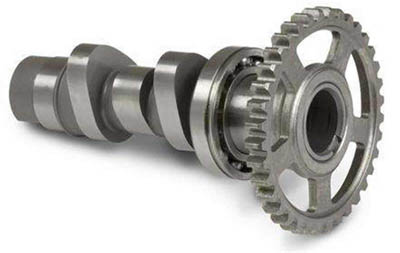
\includegraphics[width=12cm]{Immagini/camme}
	\caption{ Foto di un albero a camme.}
\end{figure}

Con parole più semplici la forma della camma rende possibile l'azionamento di una o più valvole in una determinata fase della rotazione dell'albero. 

Nel nostro caso non abbiamo camme meccaniche ne valvole ma ciò che ci interessa è il concetto che una camma ad una determinata fase della nostra macchina possa abilitare non una valvola bensì un sensore, un controllo, un comando dispositivo.

Per Camma digitale si intende dunque l'istante di attivazione di una qualunque logica programmabile. Le camme digitali vengono impostate, come anche per una camma meccanica, su un giro del motore principale.
Nel caso dell'etichettarice, ogni giro completo del motore principale corrisponde alla rotazione della stella di un unico passo (ad ogni passo di stella viene agganciato un flacone nuovo)
Possiamo perciò rappresentare un giro completo del motore principale come una "finestra" di passaggio prodotto. \textcolor{red}{IMMAGINI PER FORZA}

Per poter impostare le varie camme necessarie alla macchina necessitiamo dei gradi macchina istantanei. I gradi macchina si possono leggere mediante l'utilizzo di appositi encoder analogici, digitali oppure integrati nel motore stesso.
Una volta disponbile la lettura istantanea dei gradi macchina si possono impostare le camme digitali definendo i gradi macchina di attivazione e disattivazione. 

Un esempio semplice è quello di definire la camma di controllo presenza prodotto. Vogliamo infatti che questo controllo avvenga precisamente quando il flacone è difronte al sensore in modo da minimizzare errori di rilevamento.
Ipotizziamo ora che la posizione ottimale del flacone corrisponde a 30 gradi macchina istantanei. 
\textcolor{red}{IMMAGINI FLACONE SENSORE INGRESSO}

Possiamo creare una camma che si attiva a 20 gradi e di disattiva a 40 gradi all'interno della quale rimanere "in ascolto" del segnale del sensore per definire se il prodotto è presente o meno.

Dettagli approfonditi sull'applicazione ed implementazione delle camme digitali verranno descritti nel prossimo capitolo insieme al metodo di controllo mediante Shift Register. 

\textcolor{red}{DESCRIZIONE DI TUTTE LE CAMME DELLA MACCHINA}






\section{Controllo Mediante Shift Register}


\chapter{Protocolli di comunicazione}
Fino a qualche anno fa, i diversi fornitori di PLC mantenevano "segreti" i protocolli di comunicazione e spesso anche i Bus erano "proprietari". Anche se sugli impianti continuano a circolare decine o anche centinaia di protocolli diversi, da qualche tempo si avverte la necessità di andare verso protocolli standard. Infatti la maggior parte dei vendor ora utilizzano protocolli conosciuti che in qualche caso sono divenuti standard "di mercato" o "di fatto" (come ad esempio ModBus, Profinet, DNP3, DeviceNet, etc)
Il PLC durante il suo funzionamento può comunicare con computer, con altri PLC oppure con altri dispositivi come le macchine CNC (i torni e/o le frese a controllo numerico delle aziende). La comunicazione con computer e altri dispositivi avviene tramite tipi di connessione standard: per lo svolgimento della tesi sono stati utilizzati il protocollo Profinet e TCP.
\section{Profinet}
\textit{Profinet} \cite{profinet} è uno standard di automazione aperto che garantisce flessibilità, affidabilità
e performance.
Insieme a Profibus è un leader di mercato nel campo di azionamenti con interfacce digitali. Profinet si basa su IT-Standards, supporta TCP/IP senza limitazioni e consente l’accesso diretto dal livello di gestione aziendale fino al livello di campo. Anche l’integrazione di sistemi e di reti già esistenti non presenta alcun problema con Profinet. Profinet supporta ad esempio l’integrazione di reti Profibus e di altri sistemi di bus di campo, come AS-Interface.  
\subsection{Caratteristiche}
\begin{itemize}
	\item \textit{Safety Integrated}: Safety Integrated soddisfa tutti i requisiti	necessari per quanto concerne la sicurezza richiesta per l’uomo, la macchina e l’ambiente. Inoltre, l’utilizzo di Profinet con PROFIsafe consente di creare una rete per la comunicazione standard e orientata alla sicurezza su un solo cavo oppure anche senza fili con Industrial Wireless LAN (IWLAN);
	\item \textit{IT-Standards and Security}: Profinet offre tutte le funzioni per una configurazione e una diagnostica ottimali. Tramite Internet si può accedere a tutti i dati rilevanti da ogni luogo,in tutto il mondo. In questo Profinet soddisfa anche le crescenti esigenze per la sicurezza dei dati e della rete;
	\item \textit{Installazione della rete}: Profinet è basato con coerenza sulla tecnologia Switching a 100 Mbit/s e supporta oltre al cablaggio a stella usuale per Ethernet anche strutture di rete lineari e ad anello. Ciò riduce al minimo l’onere di cablaggio e comporta un elevato grado di flessibilità. La comunicazione senza fili mediante IWLAN offre nuove possibilità di applicazioni nell’industria, persino la funzionalità di servizio e supervisione è possibile senza fili;
	\item \textit{Comunicazione real-time}: Profinet copre l’intera gamma delle applicazioni di automazione offrendo per questo tre tipi di comunicazione di base:
	\\1. Non-Real-Time come la comunicazione TCP/IP e UDP/IP
	\\2. Real-Time (RT) e
	\\3. Isochronous Real-Time (IRT). 
	\\Profinet è quindi adatto anche per applicazioni particolarmente complesse, ad es. nel settore del Motion Control.
	\item \textit{Apparecchiature da campo decentrate}: per il collegamento diretto a Industrial Ethernet di apparecchiature da campo decentrate, \textit{Profibus and Profinet International} ha definito lo standard 'Profinet IO'. Attraverso questo standard le apparecchiature da campo trasmettono ciclicamente i dati all’immagine di processo del relativo controllore. Per l’interazione tra controllori e periferia decentrata, Profinet supporta un modello Provider/Consumer. Il Provider invia al Consumer i propri dati senza richiesta da parte del partner di comunicazione. Quest’ultimo elabora i dati. La correlazione tra Provider e Consumer è definita in fase di progettazione.
	\item \textit{Azionamenti e motion control}: Profinet riduce al minimo l’onere di cablaggio. Che si tratti di comando, operatività, accesso remoto per diagnostica e service, di parametrizzazione e messa in servizio oppure di applicazioni orientate alla sicurezza: tutti
	i compiti vengono eseguiti tramite un cavo che consente di integrare i valori di processo anche in sistemi MES ed ERP. I vantaggi risultanti sono enormi, ad esempio riguardo alla gestione dell’energia e alla manutenzione preventiva. Rende possibile, inoltre, la comunicazione wireless sulla base dei correnti standard WLAN. 
	\item \textit{Intelligenza distribuita}: Profinet offre nuove possibilità nella realizzazione di 	strutture di automazione distribuite: modularizzazione conseguente e comunicazione macchina-macchina semplificata con engineering esteso a tutto l’impianto tramite Component Based Automation.
\end{itemize}


\section{TCP}
Il \textit{Transmission Control Protocol} (TCP) \cite{TCP} è un protocollo di rete a pacchetto di livello di trasporto, appartenente alla suite di protocolli Internet, che si occupa di controllo di trasmissione ovvero rendere affidabile la comunicazione dati in rete tra mittente e destinatario. Il TCP può essere classificato al livello trasporto (OSI level 4) del modello di riferimento OSI, e di solito è usato in combinazione con il protocollo di livello rete (OSI level 3) IP. La corrispondenza con il modello OSI non è perfetta, in quanto il TCP e l'IP nascono prima del suddetto modello. I livelli TCP/IP hanno questa relazione con quelli OSI:
\begin{figure}[H]
	\centering
	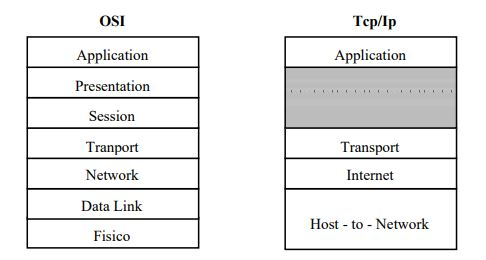
\includegraphics[width=12cm]{Immagini/1}
	\caption{ Relazione fra i livelli OSI e TCP/IP.}
\end{figure}
TCP è un protocollo orientato alla connessione e offre funzionalità di controllo di errore sui pacchetti pervenuti grazie al campo checksum contenuto nella sua PDU. Possiede inoltre funzionalità di controllo di flusso tra terminali in comunicazione e controllo della congestione sulla connessione, attraverso il meccanismo della finestra scorrevole. Questo permette di ottimizzare l'utilizzo dei buffer di ricezione/invio sui due end devices (controllo di flusso) e di diminuire il numero di segmenti inviati in caso di congestione della rete.
\\Per poter applicare il modello TCP/IP a tutti i terminali, cioè indipendentemente dal sistema operativo, il sistema di protocollo TCP/IP è stato scomposto in più moduli ciascuno con un compito preciso. Questi moduli svolgono inoltre i compiti gli uni dopo gli altri in un ordine preciso, con un sistema stratificato, ragione per cui si parla di modello a livelli. Il termine livello è usato per evocare il fatto che i dati che transitano sulla rete attraversano più livelli di protocolli. Così, i dati (pacchetti di informazioni) che circolano sulla rete sono trattati successivamente per ogni livello, che aggiunge un elemento d'informazione (detto intestazione) e poi li trasmette al livello successivo. Il modello TCP/IP è molto simile al modello OSI (con 7 livelli) che è stato elaborato dall'organizzazione internazionale degli standard (ISO, organizzazione internazionale di standardizzazione) per standardizzare le comunicazioni tra computer. 
\subsection{Server e client}
I due processi che comunicano attraverso una connessione TCP hanno ruoli diversi:
\\Il processo che avvia una nuova connessione TCP è detto client, ed invia una richiesta di connessione verso una determinata porta.
Affinché la connessione venga stabilita, su quella porta deve esserci un processo server "in ascolto", che accetta di stabilire una connessione TCP.
Le porte conosciute e registrate sono quindi utilizzate dai processi server, e sono convenzionalmente associate a particolari servizi, in modo che un client sappia a quale porta connettersi per raggiungere un determinato server.
\\Il processo server, che è in ascolto su una certa porta, rimane bloccato in attesa che un client si colleghi. Il processo client richiede di stabilire una connessione verso un determinato server su una determinata porta. Normalmente la porta sorgente usata dal client viene allocata dinamicamente dal sistema operativo del client. Quando il TCP stabilisce la connessione, a entrambi i processi viene assegnato un socket tramite cui essi possono comunicare tra loro. Tipicamente il processo server effettua una fork, affida al figlio il compito di comunicare con il nuovo client e si rimette in ascolto. Da questo punto in poi, client e server hanno ruoli simmetrici, e utilizzano gli stessi strumenti per comunicare attraverso il socket.
\subsection{Incapsulamento dei dati}
Durante una trasmissione, i dati attraversano alcuni degli strati al livello del terminale emittente. Ad ogni livello, un'informazione viene aggiunta al pacchetto di dati, si tratta di un'intestazione, un insieme di informazioni che garantisce la trasmissione. A livello del terminale ricettore, al momento del passaggio in ogni livello, l'intestazione viene letta, poi cancellata, così, alla ricezione, il messaggio è nel suo stato originale. Ad ogni livello, il pacchetto cambia aspetto, dato che gli si aggiunge un'intestazione, e quindi le denominazioni cambiano seguendo i livelli: 1) Il pacchetto di dati è detto messaggio al livello \textit{Applicazione}; 2) Il messaggio in seguito è incapsulato sotto forma di segmento nel livello \textit{Trasporto}; 3) Il segmento, una volta incapsulato, nel livello \textit{Internet} prende il nome di datagramma; 4) Infine, si parla di frame sul livello \textit{Accesso di rete}.
\subsection{Descizione livelli} 
\subsubsection{Livello Accesso di rete (host to network)}
Il livello Accesso di rete è il primo livello della pila TCP/IP capace di accedere ad una qualsiasi rete fisica, cioè rappresenta i mezzi per realizzare una trasmissione di dati attraverso una rete. Così, il livello Accesso di rete contiene tutte le specifiche riguardo la trasmissione di dati su una rete fisica, che si tratti di rete locale (Token ring, Ethernet, FDDI), di connessione ad una linea telefonica o a qualsiasi tipo di collegamento di rete. Si incarica delle nozioni seguenti: 
\begin{itemize}
	\item invio dei dati sul collegamento; 
	\item coordinamento della trasmissione dei dati (sincronizzazione); 
	\item formato dei dati; 
	\item conversione dei segnali (analogico/digitale); 
	\item controllo degl errori all'arrivo.
\end{itemize}
Fortunatamente tutte queste specifiche sono trasparenti per l'utente, dato che l'insieme di questi compiti è in effetti realizzato dal sistema operativo, come per altro i driver dell'hardware che permettono la connessione alla rete (ad esempio driver della scheda di rete).
\subsubsection{Il livello Internet}
Il livello internet è il livello "più importante" (sono tutti importanti) dato che è quello che definisce i datagrammi, e che gestisce le nozioni d'indirizzamento IP. Esso permette l'invio dei datagrammi (pacchetti di dati) verso dei terminali remoti nonché la gestione della loro frammentazione e riassemblaggio alla ricezione. 
\subsubsection{Il livello di trasporto}
I protocolli dei livelli precedenti permettevano di inviare delle informazioni da un terminale all'altro. Il livello Trasporto permette a delle applicazioni che girano su terminali remoti di comunicare. Il problema consiste dell'identificare queste applicazioni. In effetti, a seconda del terminale e del suo sistema operativo, l'applicazione potrà essere un programma, un compito, un processo, ecc. Inoltre, la denominazione dell'applicazione può variare da un sistema all'altro, ed è la ragione per cui un sistema di numero è stato realizzato per poter associare un tipo di applicazione ad un tipo di dati; questi identificativi sono detti porte. Il livello Trasporto contiene due protocolli che permettono alle due applicazioni di scambiare dei dati indipendentemente dal tipo di rete scelta (cioè indipendentemente dai livelli inferiori, ecc.). Si tratta dei seguenti protocolli: TCP, un protocollo orientato connessione che assicura il controllo degli errori; UDP, un protocollo senza connessione il cui controllo d'errore è obsoleto. 
\subsubsection{Il livello applicazione}
Il livello Applicazione è quello situato alla sommità dei livelli dei protocolli TCP/IP. Esso contiene le applicazioni di rete che permettono di comunicare grazie ai livelli inferiori. I software di questo livello comunicano quindi grazie ad uno dei due protocolli del livello inferiore (il livello trasporto) cioè TCP o UDP. 
\\Le applicazioni di questo livello sono di differenti tipi, ma la maggior parte sono dei servizi di rete, cioè delle applicazioni fornite all'utente per assicurare l'interfaccia con il sistema operativo. Possiamo classificarli secondo i servizi che offrono: servizi di gestione (trasferimento) di file e di stampa, servizi di connessione alla rete, servizi di connessione remota, le diverse utility di Internet (figura \ref{1}). 
\begin{figure}[H]
	\centering
	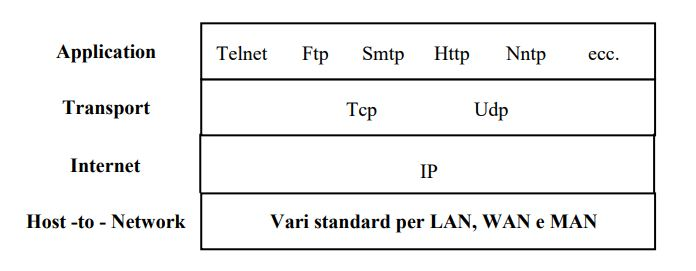
\includegraphics[width=12cm]{Immagini/2}
	\label{1}
	\caption{ Relazione fra i livelli e protocolli dell'architettura TCP/IP.}
\end{figure}

\section{Open Platform Communications (OPC)}
OPC \cite{OCP} è lo standard di interoperabilità per lo scambio sicuro e affidabile di dati nello spazio di automazione industriale e in altri settori. È indipendente dalla piattaforma e garantisce il flusso continuo di informazioni tra i dispositivi di più fornitori. La Fondazione OPC è responsabile dello sviluppo e della manutenzione di questo standard.
Lo standard OPC è una serie di specifiche sviluppate da venditori del settore, utenti finali e sviluppatori di software. Queste specifiche definiscono l'interfaccia tra client e server, nonché server e server, compreso l'accesso ai dati in tempo reale, il monitoraggio di allarmi ed eventi, l'accesso ai dati storici e altre applicazioni.
\\Quando lo standard fu rilasciato per la prima volta nel 1996, il suo scopo era quello di astrarre protocolli specifici del PLC (come Modbus, Profibus, ecc.) In un'interfaccia standardizzata che permettesse ai sistemi HMI / SCADA di interfacciarsi con un "uomo medio" che convertisse generico- OPC leggere / scrivere richieste in richieste specifiche del dispositivo e viceversa. Di conseguenza, è emersa un'intera industria di prodotti artigianali che consente agli utenti finali di implementare sistemi che utilizzano i migliori prodotti interagendo perfettamente tramite OPC.
\\Inizialmente, lo standard OPC era limitato al sistema operativo Windows. Come tale, l'acronimo OPC è stato generato da OLE (object linking and embedding) per Process Control. Queste specifiche, che ora sono conosciute come OPC Classic, hanno goduto di un'adozione diffusa in diversi settori, tra cui produzione, automazione degli edifici, petrolio e gas, energie rinnovabili e servizi pubblici, tra gli altri.
\\Con l'introduzione di architetture orientate ai servizi nei sistemi di produzione sono arrivate nuove sfide nella sicurezza e nella modellazione dei dati. La OPC Foundation ha sviluppato le specifiche OPC UA per soddisfare queste esigenze e, allo stesso tempo, ha fornito un'architettura a piattaforma aperta ricca di funzionalità che era a prova di futuro, scalabile ed estensibile.
\\Oggi l'acronimo OPC sta per Open Platform Communications.
\\Questi sono solo alcuni dei motivi per cui così tanti membri e altre organizzazioni tecnologiche (collaborazioni) si stanno rivolgendo a OPC UA per la loro piattaforma di interoperabilità.
\subsection{Architettura client/server}
OPC si presenta come un’architettura client/server che permette ad un qualsiasi processo (Client) basato su OPC di accedere a qualsiasi sorgente di dati (Server) dotata di interfacce OPC. I fornitori hardware offrono un Server OPC, che permette a qualsiasi applicazione Client di accedere ai dati da esso pubblicati. I server OPC forniscono un metodo per molti pacchetti software diversi (purché si tratti di un client OPC) per accedere ai dati da un dispositivo di controllo del processo, come un PLC o un DCS. Tradizionalmente, ogni volta che un pacchetto richiedeva l'accesso ai dati da un dispositivo, un'interfaccia personalizzata o un driver, doveva essere scritto. Lo scopo di OPC è definire un'interfaccia comune che venga scritta una sola volta e quindi riutilizzata da qualsiasi business, SCADA, HMI o pacchetti software personalizzati.
\\Una volta che un server OPC è stato scritto per un particolare dispositivo, può essere riutilizzato da qualsiasi applicazione in grado di agire come client OPC. I server OPC utilizzano la tecnologia OLE di Microsoft (nota anche come Component Object Model o COM) per comunicare con i client. La tecnologia COM consente di definire uno standard per lo scambio di informazioni in tempo reale tra applicazioni software e hardware di processo.
\\È importante notare che alcune specifiche OPC sono pubblicate, altre sono disponibili solo per i membri della OPC Foundation. Quindi, mentre nessuna azienda "possiede" OPC e chiunque può sviluppare un server OPC, indipendentemente dal fatto che siano o meno membri della OPC Foundation, i non membri non utilizzeranno necessariamente le specifiche più recenti. Chiunque può integrare i prodotti OPC e non esiste alcun pre-requisito per l'integratore di sistemi di appartenere a qualsiasi organizzazione. Spetta quindi a ciascuna società che richiede prodotti OPC di garantire che i propri prodotti siano certificati e che i loro integratori di sistemi dispongano della formazione necessaria.
In figura \ref{OPC} è possibile osservare le percentuali dei campi di utilizzo di OPC.
\begin{figure}[H]
	\centering
	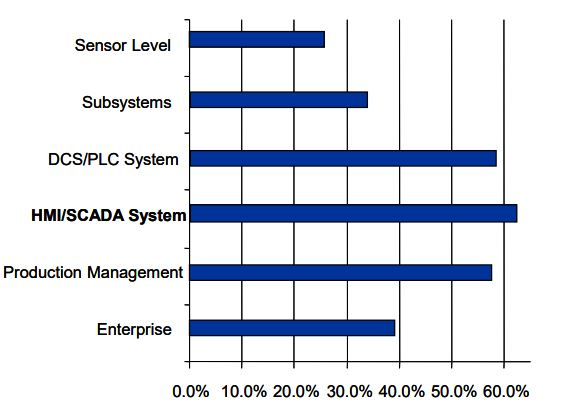
\includegraphics[width=13cm]{Immagini/OPC}
	\label{1}
	\caption{Campi di utilizzo OPC.}
\end{figure}
\subsection{Unified Architecture}
Nella tesi è stata usata la versione Unified Architecture: OPC Unified Architecture (UA), pubblicato nel 2008, è un'architettura orientata ai servizi indipendente dalla piattaforma che integra tutte le funzionalità delle singole specifiche OPC Classic in un unico framework estendibile. Questo approccio a più livelli raggiunge gli obiettivi di specifiche di progettazione originali di:
\begin{itemize}
	\item \textit{Equivalenza funzionale}: basandosi sul successo di OPC Classic, OPC UA è stato progettato per migliorare e superare le capacità delle specifiche OPC Classic. OPC UA è funzionalmente equivalente a OPC Classic, ma capace di molto di più (ad esempio trova la disponibilità di OPC Server su PC e / o reti locali, o ancora permette di leggere e scrivere dati/informazioni in base alle autorizzazioni di accesso).
	\item \textit{Indipendenza dalla piattaforma}: da un microcontroller incorporato a un'infrastruttura basata su cloud; OPC UA fornisce l'infrastruttura necessaria per l'interoperabilità in tutta l'azienda, da macchina a macchina, da macchina a impresa e tutto ciò che è intermedio.
	\item \textit{Sicuro}: una delle considerazioni più importanti nella scelta di una tecnologia è infatti proprio la sicurezza. OPC UA è adatto al firewall e risolve i problemi di sicurezza fornendo una suite di controlli mediante crittografia, autenticazione e auditing.
	\item \textit{Estendibile}: possibilità di aggiungere nuove funzionalità senza influire sulle applicazioni esistenti; l'architettura multistrato di OPC UA offre una struttura "a prova di futuro". Tecnologie e metodologie innovative come nuovi protocolli di trasporto, algoritmi di sicurezza, standard di codifica o servizi applicativi possono essere incorporati in OPC UA mantenendo la retrocompatibilità per i prodotti esistenti.
	\item \textit{Modellazione completa delle informazioni}: la struttura di modellazione delle informazioni di OPC UA trasforma i dati in informazioni. Con capacità complete orientate agli oggetti, anche le strutture multi-livello più complesse possono essere modellate ed estese. I tipi di dati e le strutture sono definiti nei profili. Ad esempio, le specifiche OPC Classic esistenti sono state modellate in profili UA che possono essere estesi anche da altre organizzazioni (fig \ref{OPC2}).
	\begin{figure}[H]
		\centering
		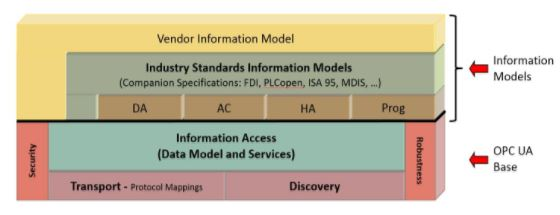
\includegraphics[width=13cm]{Immagini/OPC2}
		\label{OPC2}
		\caption{Estensione modello.}
	\end{figure}
\end{itemize}

\chapter{Schema generale di comunicazione}
Disegno che mostra lo schema di comunicazione tra i vari dispositivi (MAGARI DA TIA PORTAL)
\section{Profinet Mitsubishi}
Registro di comunicazione e FB di controllo
\section{Profinet Datalogic}
Registro di comunicazione e FC di controllo
\section{TCP Stampante VideoJet}

\chapter{HMI/SCADA}
Un HMI, o interfaccia uomo-macchina, è un dispositivo o un software che permette al suo utilizzatore di comunicare con un macchinario o un impianto di produzione. Come? Traducendo una quantità immensa di dati complessi in informazioni accessibili all’uomo. In questo modo l’operatore ha a sua disposizione tutti gli strumenti necessari per controllare il processo di produzione.
Contestualizzando questa definizione nel mondo dell’Automazione Industriale, risulta dunque evidente che più intuitivo e user-friendly è l’HMI, più efficiente e redditizio risulta il lavoro.

Sostanzialmente un dispositivo HMI rende possibile la visualizzazione e il controllo delle applicazioni. Sfruttando risorse come I/O, SoftPlc CoDeSys o Ethercat e sistemi operativi (ancora meglio se embedded), permette di comunicare con qualsiasi sistema aziendale.


\section{HMI dell'Etichettatrice}
Asem da 11 pollici con windows 7 embedded ecc ecc
\section{Tool Sviluppo}
\section{Industria 4.0}
\subsection{OPC}
\subsection{RealTime Sql DataBinding}
\subsection{Reporting Server}
\subsection{SCADA Web Interfaces}

\section{Code of Federal Regulations Title 21}
\subsection{Specifiche 21CFR}
\subsection{Realizzazione}






\newpage
\begin{thebibliography}{100}
	\bibitem{profinet}
	'Automatizzare e trarre immediato profitto con lo standard leader Industrial Ethernet.'\url{http://w5.siemens.com/italy/web/AD/ProdottieSoluzioni/Sistemiautomazionenew/homepageProfinet/Documents/Brochure_PROFINET.pdf}	
	
	\bibitem{TCP}
	L. Parziale et al:'TCP/IP Tutorial and Technical Overview' IBM RedBooks, December 2006
	
	\bibitem{OCP}
	\url{https://opcfoundation.org/}
	
	
	

	
\end{thebibliography}
\end{document}
